\section{Gallery}
\label{sec:vis_gallery}

\begin{figure}[htb]
\begin{center}
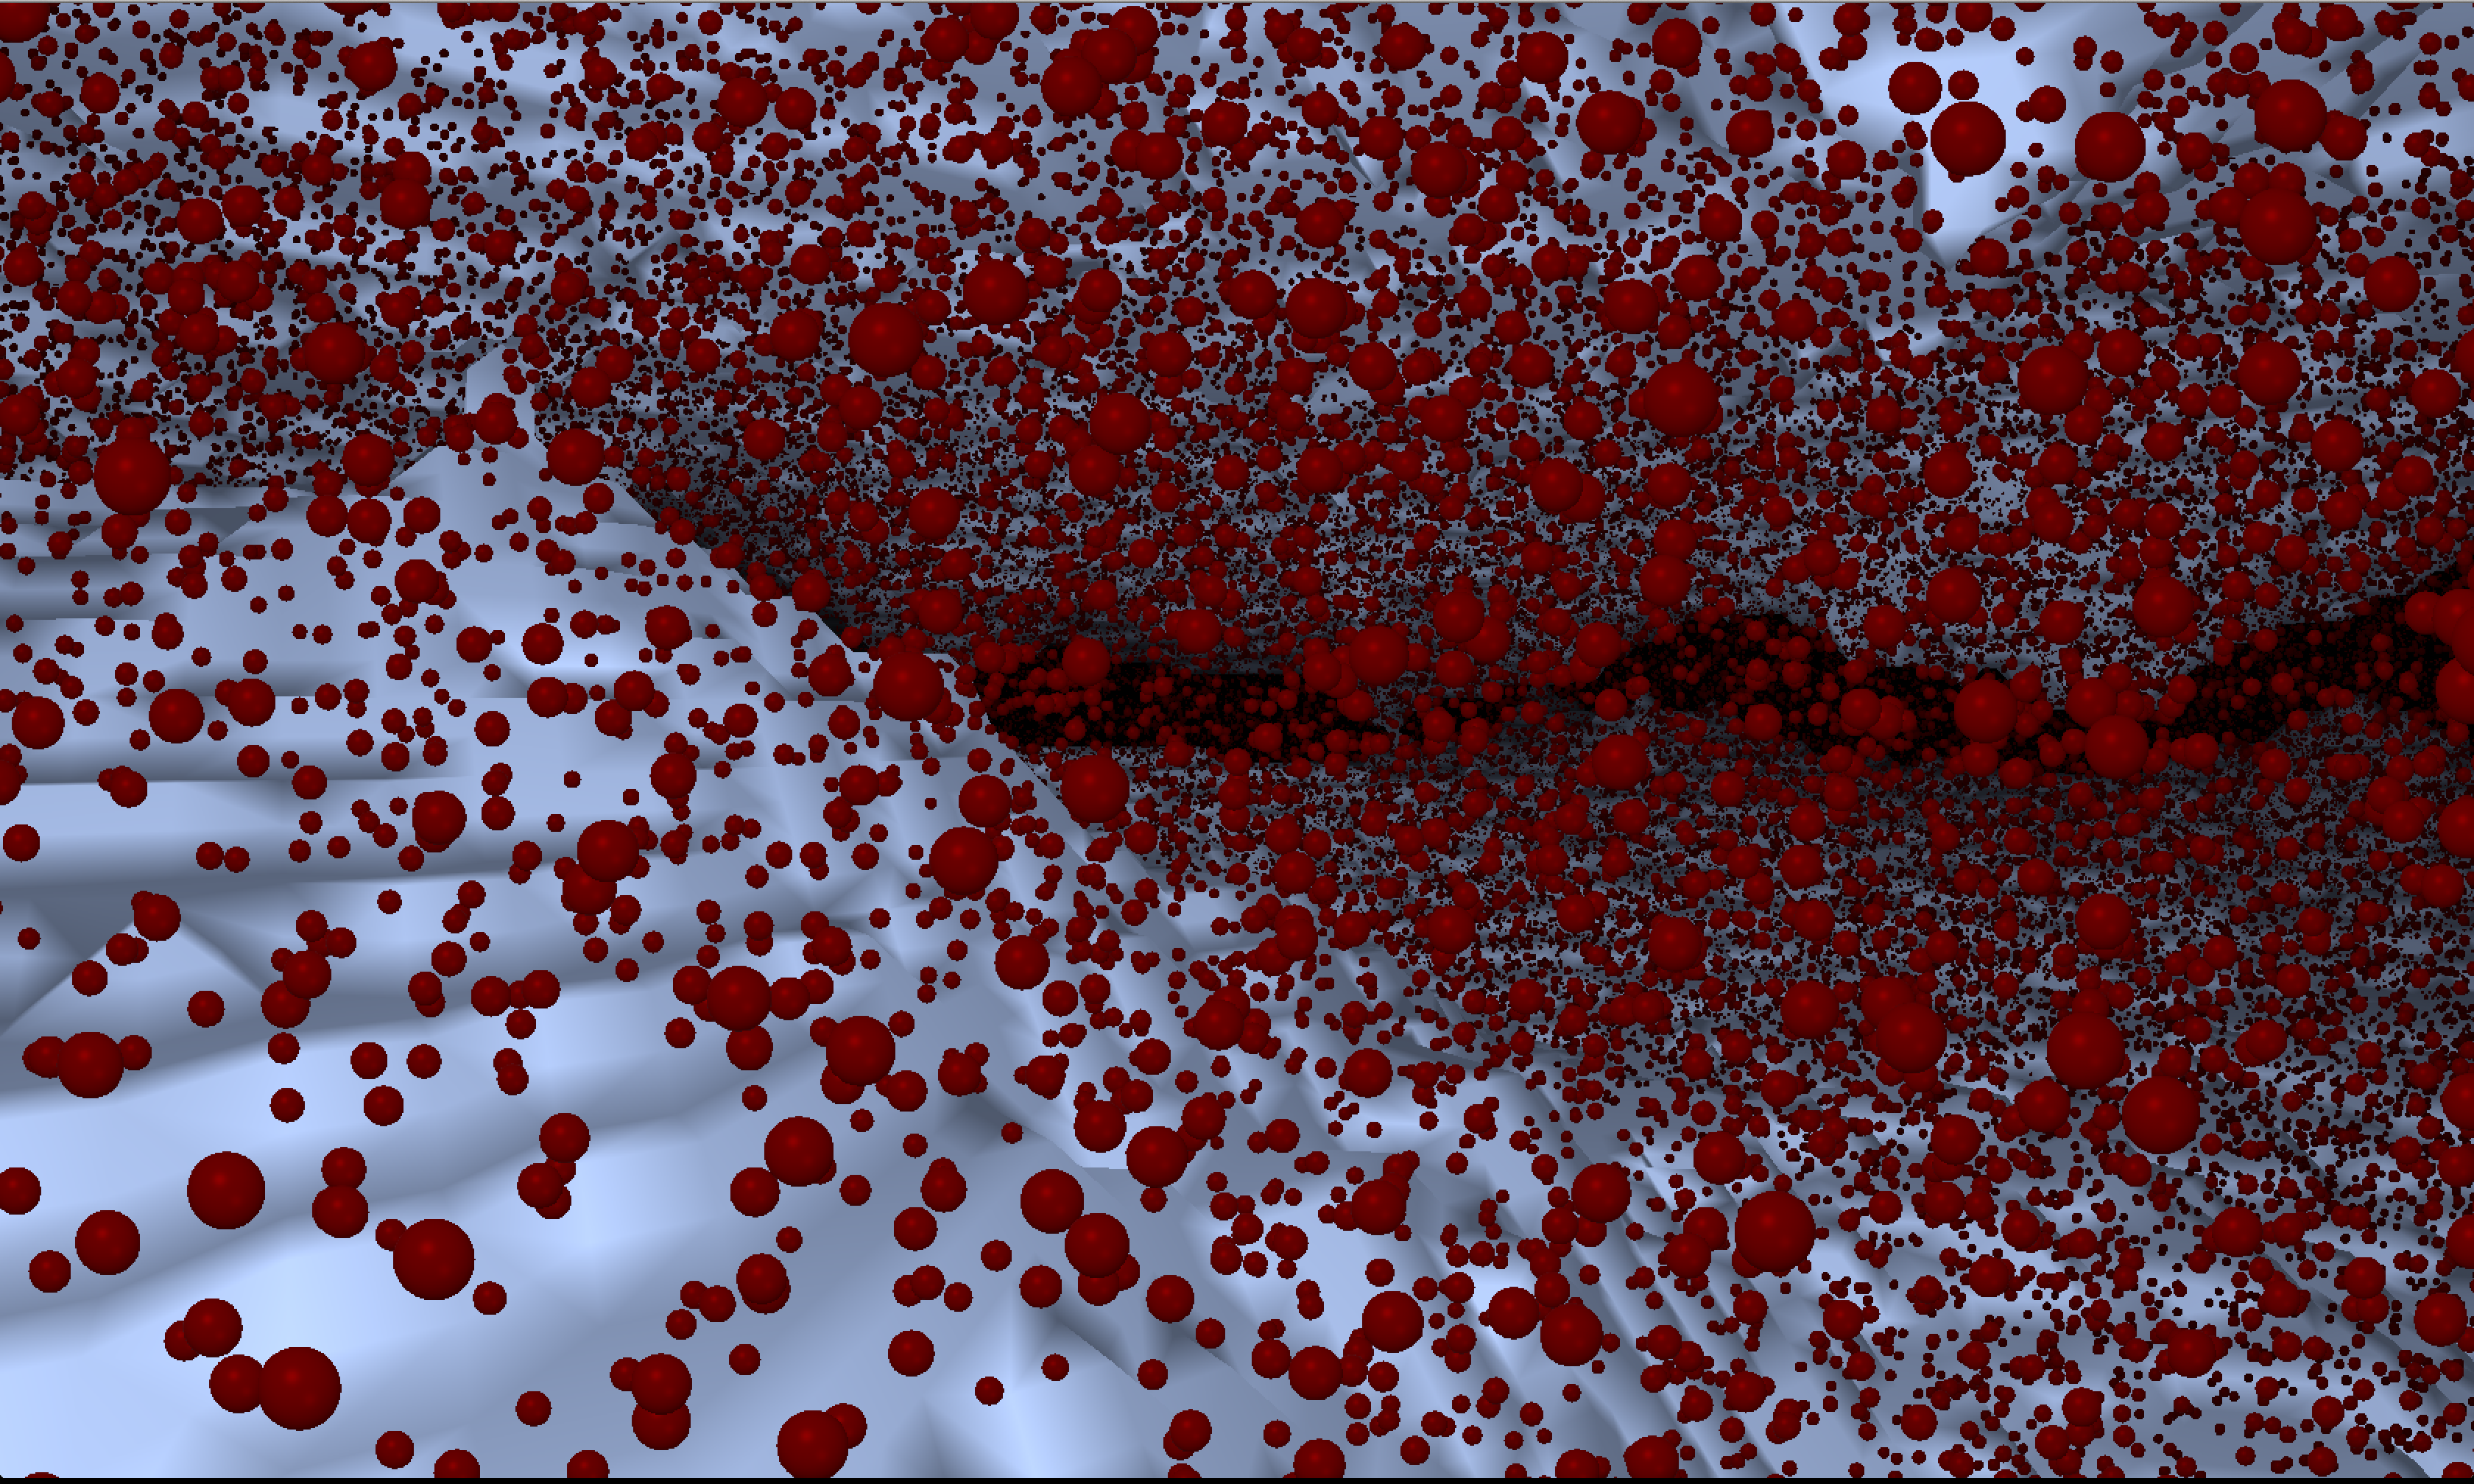
\includegraphics[width=0.8\textwidth, trim=0cm 0cm 0cm 0cm, clip]{visualization/figures/marching_cubes_fracture.png}
\end{center}
\caption{A cube consisting of eight vertices. Given that each vertex can have a value smaller or larger than some given iso-value, the cube has has $2^8=256$ different combinations. This number can, as we see here, be reduced to 15 due to symmetries. An iso-surface on a scalar field can then be generated as renderable triangles with this technique. Image from \url{http://en.wikipedia.org/wiki/File:MarchingCubes.svg}, accessed 20 March, 2014.}
\label{fig:vis_marching_cubes}
\end{figure}
